% \documentclass[sort&compress]{elsarticle}
\documentclass[final,3p,times,twocolumn,sort&compress]{elsarticle}
%\documentclass[review]{elsarticle}


\usepackage{lineno,hyperref}
\modulolinenumbers[2]

\journal{Remote Sensing of Environment}

%% Packages
\usepackage{tabu}
\usepackage{breakurl}
\usepackage{float}

%%%%%%%%%%%%%%%%%%%%%%%
%% Elsevier bibliography styles
%%%%%%%%%%%%%%%%%%%%%%%
%% To change the style, put a % in front of the second line of the current style and
%% remove the % from the second line of the style you would like to use.
%%%%%%%%%%%%%%%%%%%%%%%

%% Numbered
% \bibliographystyle{model1-num-names}

%% Numbered without titles
%\bibliographystyle{model1a-num-names}

%% Harvard
% \bibliographystyle{model2-names.bst}\biboptions{authoryear}

%% Vancouver numbered
% \usepackage{numcompress}\bibliographystyle{model3-num-names}

%% Vancouver name/year
% \usepackage{numcompress}\bibliographystyle{model4-names}\biboptions{authoryear}

%% APA style
%\bibliographystyle{model5-names}\biboptions{authoryear}

%% AMA style
% \usepackage{numcompress}
% \bibliographystyle{model6-num-names}

%% `Elsevier LaTeX' style
\bibliographystyle{elsarticle-num}

%%%%%%%%%%%%%%%%%%%%%%%

\begin{document}

\begin{frontmatter}

\title{Night and day: What are the nonlinear associations between urban characteristics and land surface temperature?}

%% or include affiliations in footnotes:
\author[1]{T.M. Logan\corref{mycorrespondingauthor}}
\cortext[mycorrespondingauthor]{Corresponding author}
% \ead[url]{www.tomlogan.co.nz}
\ead{tom.logan@canterbury.ac.nz}

\author[2]{B. Zaitchik}
\author[1]{S. Guikema}
\author[]{A. Nisbet}


\address[1]{Industrial and Operations Engineering, University of Michigan, Ann Arbor, MI}
\address[2]{Earth and Planetary Sciences, Johns Hopkins University, Baltimore, MD}

\begin{abstract}
Although heat waves and the urban heat island are nocturnal phenomena, the drivers of land surface temperature during the night remain poorly understood.
Understanding these drivers is necessary for reducing land surface temperature and mitigating heat waves, the deadliest natural hazard, which are expected to increase in frequency and severity.
% However, only recently has nocturnal imagery become available from LandSat allowing nighttime land surface temperature to be analyzed.
However, the independent effects and relative importance of potential drivers remain unclear from existing studies.
We seek to answer the question: ``What is the relative importance and nonlinear affects of urban characteristics associated with land surface temperature during both the day and night?'' 
To do this, we analyze the urban land surface temperature in four cities across the United States.
In our analysis, we include variables related to vegetation, water, the built-environment, and topography. 
We control these variables using nonlinear statistical methods which allow for their independent effects to be assessed.
The effects from the daytime and nighttime analysis are compared to determine if previously reported relationships hold between cities and during both the day and night.
Understanding the relationships influencing both night and day land surface temperature will improve climate adaptation planning and heat wave mitigation.
\end{abstract}

\begin{keyword}
Urban climate; LandSat; Land surface temperature; Urban canyon; Machine learning; Convolutional Neural Network
\end{keyword}

\end{frontmatter}

\linenumbers

\section{Introduction}
In a warming world, understanding the drivers of high land surface temperature (LST) and the urban heat island (UHI) will aid in adapting cities in mitigating urban heat for the health and well being of their communities.
And mitigate they must; the 1995 Chicago heat wave, which killed more than 700 people,\footnote{The 2003 European heatwave killed 70,000 \cite{Robine2008-ky} and the 2015 European heat wave increased mortality up to 30\% \cite{Vicedo-Cabrera2016-si}} is expected to become an annual occurrence by 2080 \cite{klinenberg2015heat}. 
Heat waves' affect on people is exacerbated by the urban heat island (UHI) \cite{Wicki2017-fv, Echevarria_Icaza2016-fr}.
The UHI results from heat captured during the day being released during the night, thus increasing nocturnal temperatures \cite{Oke2002-ta, Landsberg1981-mq, Rotach2005-yu}.
This increase in nocturnal temperature reduces people's ability to cool off during the night and drives an increase in mortality \cite{Echevarria_Icaza2016-fr, Murage2017-wj}.

Urban heat is studied in two ways.
The first uses weather station data to analyze air temperature (e.g. \cite{Scott2016-lc}) while the other uses remote sensing to examine the land surface temperature (LST) \cite{Imhoff2010-lf, Peng2012-iy, Peng2018-cp, Zhou2014-wc, Voogt2003-mm}.
Although there are differences between LST and air temperature \cite{Good2016-yk}, the extensive spatial coverage of LST data is a major advantage and enables comparative studies \cite{Hung2006-qy}.
We analyze LST in this study.

Most existing LST studies focus on the daytime \cite{Peng2018-cp,Chun2018-so,Wang2019-water,Zhou2018-iy}.
However, the mechanisms and urban characteristics driving LST allegedly differs between night and day \cite{Hung2006-qy, Chun2017-mm, Nichol2005-mm, Wicki2017-fv, Echevarria_Icaza2016-fr,Sobstyl2018-wt, Peng2012-iy, Zhou2014-wc, Zhao2017-cc}. 
Given that UHI is a nocturnal phenomena, the lack of study on nighttime LST leaves a critical gap in our understanding. 
This can now be addressed as high resolution nighttime satellite images have become available.

Existing studies that have analyzed LST have used low-resolution imagery, making it challenging to deduce a clear understanding of the the influence and relative importance of the associated urban characteristics \cite{Chun2017-mm, Echevarria_Icaza2016-fr, Wicki2017-fv, Zhou2014-wc}. 
Additionally, these studies can be enhanced by: 1) studying multiple regions, 2) considering 2D and 3D urban characteristics, 3) improving their statistical techniques.
The data availability has limited previous nocturnal studies, meaning that many rely on MODIS images with a 1km resolution \cite{Zhou2014-wc, Echevarria_Icaza2016-fr,Wang2019-tree,Peng2012-iy}.
1km resolution makes it difficult to attribute LST to urban characteristics.
However, 30-m resolution LandSat8 (L8) night scenes have recently become available. 
Due to the wide spatial availability of L8 imagery, comparative studies between cities, necessary to understand the generalizability of findings \cite{Peng2012-iy, Hung2006-qy}, can now be conducted for day and night.

Existing studies have also been criticized for the explanatory variables they've used \cite{Chun2017-mm,Peng2018-cp}.
There is ongoing disagreement regarding the importance of 3D (e.g. building height) vs 2D (such as albedo) variables.  
Competing studies suggest that 3D factors are not important \cite{Berger2017-lx}, while others find that ignoring 3D incorrectly conflates the effect of different 2D variables \cite{Chun2017-mm}.
Beyond the 2D or 3D debate, five categories of important variables have been identified: Green space, water, landscape, albedo, and socio-economic \cite{Peng2018-cp}. 
However, many studies do not capture these categories and, worse, many analyze only the single effect of each variable \cite{Zhao2017-cc, Merbitz2012-xz, Unger2004-ry} (see \cite{Peng2018-cp, Chun2017-mm} for further discussion). 
Considering a variable in isolation, without accounting for potential conflating by other variables, limits the understanding of the interdependent effects that exist.

The third potential enhancement is in the statistical approaches.
Almost all studies use linear techniques (e.g. \cite{Li2017-yl, Peng2012-iy, Wicki2017-fv,Zhou2014-wc,Peng2018-cp,Echevarria_Icaza2016-fr,Chun2017-mm,Chun2018-so,Wang2019-tree,Wang2019-water}.
Using linear models incur a number of major challenges that limit these studies' ability to explain the interdependencies between variables. 
The first is that many of the urban characteristics exhibit high multicollinearity \cite{Zhou2014-wc}.
The second is that linear models are limited in their ability to quantify the independent effects of characteristics and their relative influence on LST \cite{Peng2018-cp, Zhou2014-wc}.
Additionally, and most importantly, these studies only assess their accuracy using in-sample validation techniques.
In-sample validation means that model accuracy is assessed with the same data used in the training, rather than unseen data. 
This risks overestimating the accuracy of their models.

The question we address is: ``What is the relative importance and nonlinear affects of urban characteristics associated with land surface temperature during both the day and night?''
To achieve this we conduct a comparative study of four cities in the United States using non-linear statistical techniques which capture the interdependencies and relative importance between the urban characteristics.
In addressing our question, we will address the, at times fundamental, limitations of existing studies.
Most importantly we look at nighttime temperature as well as daytime, we appropriately validate our statistical models, and we use tools that allow us to explore the interdependent effects of urban characteristics on urban heat.
The results have implications for mitigating the severity of future heat waves.

\section{Data and Methods}
\subsection{Cities studied}

We study four cities in the contiguous United States (Figure \ref{fig:map}): Baltimore, MD; Detroit, MI; Phoenix, AZ; and Portland, OR. These four cities were selected as they include East and West coast cities, a mid-western city, and an arid central city. Phoenix, additionally, has been the subject of numerous other studies on land surface temperature. The cities were also selected due to lidar availability which is required for calculating the 3D variables. The constraint on selecting more cities was the time and computational requirements primarily for the LST and sky view factor calculations. 

Figure \ref{fig:map} shows the gridded LST data for each of the cities and Figure \ref{fig:joy} shows the distribution of each city's day and night land surface temperature. 

\begin{figure*}
    \centering
    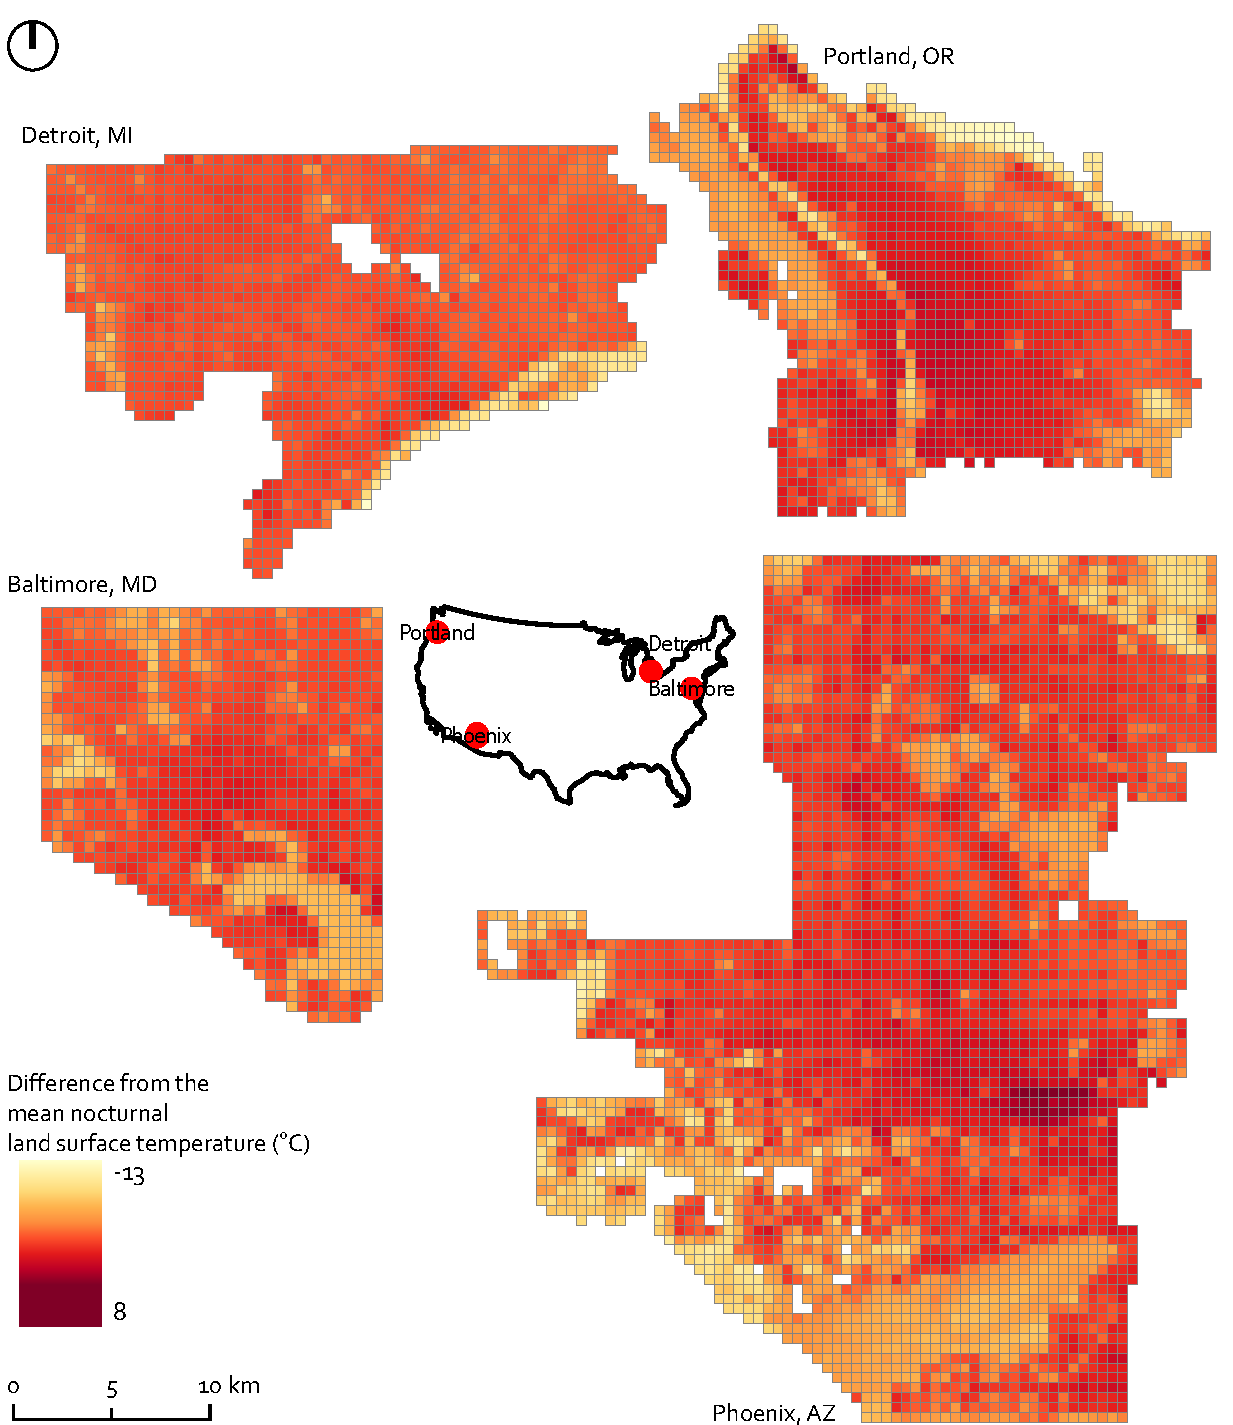
\includegraphics[width=\textwidth]{fig/report/map_nocturnal_lst.pdf}
    \caption{The gridded nocturnal land surface temperature in $^o$C of the cities studied. This is change from the mean (average) for each city.}
    \label{fig:map}
\end{figure*}


\begin{figure}
    \centering
    \includegraphics[width=\linewidth]{fig/report/joyplot_lst_500.pdf}
    \caption{The distribution of nocturnal and diurnal land surface temperature of the cities studied.}
    \label{fig:joy}
\end{figure}

\subsection{Land surface temperature}
We calculate land surface temperature using Landsat 8 (Land Processes Distributed Active Archive Center product) imagery, land cover data, and an air temperature observation (data sources provided in \ref{tab:data}). 
Our code is available on our Github\footnote{URL redacted for review} repository, and is as follows:
We convert Band-10 digital-number data to top-of-atmosphere radiance \cite{Jimenez-Munoz2003-wc}. 
We correct for emissivity using land cover data \cite{Alipour2003-gb}, and then calculate the at-satellite brightness temperature \cite{Jimenez-Munoz2003-wc}. 
Finally an atmospheric correction is made as per the monowindow algorithm \cite{Qin2001-jn} using the maximum observed temperature of the day from a nearby weather station. 
This follows the process is described in \cite{Scott2016-lc}. 

To ameliorate the effect of shadows and other ephemeral changes \cite{Zhou2018-iy} we use at least three minimal-cloud images for each city and night/day period and calculate the mean of LST.

So we can conduct the comparative study between the cities, the land surface temperature for each city is calculated as the difference from the city's mean. 

\begin{figure}
    \begin{center}
    \includegraphics[width=\linewidth]{fig/report/scatter_500.png}
    \caption{The land surface temperature in $^o$C of the cities studied at a 500m square resolution.}
    \label{fig:scatter_lst}
    \end{center}
\end{figure}

\subsection{Independent variables}

\textit{Albedo}. Albedo is a measure of the reflectivity or brightness of a surface. It is normalized between 0-100 where the darker surfaces are lower values. Albedo is calculated using the LandSat8 images using the algorithm described in \cite{Smith2010-nw, Liang2001-jd}. 

\textit{Building floor area}. The building floor area within the cell. This uses data released in 2018 by Microsoft where building footprints are estimated using areal images. 

% \textit{Building height}. Building height is estimated using the building footprints and available lidar data following \cite{Chun2017-mm}. The mean lidar elevation within each building's footprint is subtracted by the mean digital elevation (topography) within the footprint to estimate the building's height.

\textit{Elevation}. 1/3 arc-second (~10m) bare-earth elevation (topography) data is available courtesy the U.S. Geological Survey. 

\textit{Surface elevation}. The surface elevation is determined from the lidar data. Surface elevation captures the natural and built features. 

\textit{Impervious surface percentage}. This is provided in the National Land Cover Database from the Multi-Resolution Land Charasteristic Consortium \cite{Xian2011-aa}. To generate the impervious surface area (ISA) LandSat data, NLCD land cover, and nighttime light imagery is used. The stable nighttime light intensity is only used to estimate the boundary of of urban areas. The Landsat images were converted to top-of-atmosphere reflectance. The data is provided at a 30m resolution.

\textit{Land cover}. 
Classification of land cover is described in \cite{Homer2015-ce}. 
However, as it is used in the calculation of emissivity when calculating the LST it cannot be used as an independent variable. 
The only landcover that we use is category 11, water. 

\textit{NBDI}. 
Normalized difference built-up index indicates the intensity of imperviousness \cite{Bhatti2014-ae}. 
It is calculated from satellite images as $$NDVI=\frac{B_{SWIR}-B_{NIR}}{B_{SWIR}+B_{NIR}}$$ where $B_{NIR}$ and $B_{SWIR}$ are the reflectances in the near-infrared and short-wave infrared bands respectively \cite{Alhawiti2016-wv}. 
Using LandSat8 imagery, this is $$NDVI=\frac{B6-B5}{B6+B5}$$ \cite{barsi2014}.
% *Kaplan 2018, Peng 2018

\textit{NDVI}. 
The normalized difference vegetation index (NDVI) measures green vegetation. 
It is calculated from satellite images as $$NDVI=\frac{B_{NIR}-B_{red}}{B_{NIR}+B_{red}}$$ where $B_{NIR}$ and $B_{red}$ are the reflectances in the near-infrared and red bands respectively \cite{Alhawiti2016-wv}. 
Using LandSat8 imagery, this is $$NDVI=\frac{B5-B4}{B5+B4}$$ \cite{barsi2014}.

% \textit{Nighttime light intensity}. Stable nighttime light intensity is available from the Defense Meteorological Satellite Program (DMSP) Operational Linescan System (OLS). They prepare the data to remove clouds and ephemeral light sources. We use 2013 (the most recently available) data of version 4 at a spatial resolution of 30 arc-seconds (1km at the equator) \cite{ngdc2013version}. The nighttime light intensity was found to be only in moderate agreement with density \cite{bagan2018}, meaning lights may indicate anthropogenic energy use during the night. However, it's lower resolution means that can not capture minor differences. We resampled the raster to a 30m resolution, as per the NLDC \cite{Homer2015-ce}, and for each grid calculated the mean, min, and max.

\textit{Population density}. 
Density allegedly increases the LST \cite{Li2017-yl, Peng2018-cp}, although this result may be the result of confounding with other factors. 
Population density is calculated from the U.S. census at the block level. 
The most recent census was 2010, so we use that data as an estimator of where people reside in the evening. 
This data is also at a lower resolution that the grid cells used, so the grid cell assumes the density of the block that it's centroid is contained within.

\textit{Sky view factor}. Urban canyons have been found to have an effect on UHI because they prevent air circulation \cite{Landsberg1981-mq, Chun2017-mm} and are used to indicate radiation flux within complex environments \cite{Matzarakis2007-xy}. We calculate SVF using \cite{Van_doninck2018-ib} and following the parameters used by \cite{Chun2017-mm}: the number of search directions, $\phi=10^o$; and the radius of the reference circle, $R=300m$. We use a spatial resolution of 6 meters.
% * Yuan 2011, Unger 2004.

\textit{Tree canopy cover}. 
The percent tree canopy cover is calculated using National Agriculture Imagery Program (NAIP) aerial imagery, Landsat 5 imagery, elevation, and existing NLCD data \cite{Coulston2012-uu, Homer2015-ce}. 
The data provided is at a 30m resolution. 
The six reflective bands from Landsat 5 are used to calculate top-of-atmosphere reflectance \cite{Coulston2012-uu} so the data does not contain information used in the LST calculation (which requires radiance). 
% * Rogan 2013, Elmes 2017

\subsection{Data preparation and robustness}
\begin{figure*}
    \centering
    \includegraphics[width=\linewidth]{fig/report/holdout_500.png}
    \caption[Holdout cross-validation results at 500 meter resolution]{
    The out-of-bag (OOB) R$^2$ and mean absolute error (MAE) of the models from a 100-fold holdout cross-validation. 
    The models were trained on 80\% of the data and tested on the unseen 20\%.
    When selecting data for the training and testing sets, spatial subsets were used to account for spatial similarities. 
    OOB R$^2$ can vary between $(-\infty, 1)$, where better models have a value near 1. 
    Good models have MAE near 0.
    }
    \label{fig:holdout_500}
\end{figure*}

The objective of our study is to determine the most influential urban characteristics and understand how they relate to land surface temperature.
To do this, we use partial dependence plots to understand how the urban characteristics are associated with land surface temperature.
Given a dataset and for a chosen characteristic, partial dependence is calculated by fixing the value of that characteristic in all observations in the dataset and predicting the land surface temperature. 
This is repeated over a range for the feature of interest.
To evaluate how multiple urban characteristics interact, partial dependence can also be conducted in multiple dimensions.
The swing \cite{Shortridge2015-ub} measures the relative importance of variables by calculating the magnitude of change in temperature associated with each variable.
To calculate partial dependence, we need a data set and a statistical model.

To analyze the data, it needs to transformed into a spatially consistent set.
The raw data is a variety of spatial data types from area level (the population density data), to geostatistical raster (e.g. the land surface temperature).
We choose to resample the data into a grid of square cells.
We conduct the resampling twice to produce a grid of 500m and 100 meter cells. 
Having two grid resolutions allowed us to ensure our conclusions are robust.
For each of the cells the the mean, maximum, and minimum of all variables were calculated. 
To further account for spatial effects of each variable, the mean of the surrounding cells (including diagonal) was calculated and the resulting spatial lag variable was included as an additional independent variable. 
To address multicollinearity between the variables, that would confound our analysis of influence, we remove variables iteratively that have a Variance Inflation Factor greater than approximately 5.
The result is a data set which with we can train a variety of statistical models.

Various statistical models (\S \ref{ss:models}) were trained and then, crucially, validated on unseen data using a technique known as holdout cross-validation. 
This approach partitions 80\% of the data into a training set and the remaining 20\% into the testing set.
The model resulting from the training, is then tested on this unseen test set (known as out-of-bag), to get an estimate of the model accuracy.
This is repeated 100 times and the distribution of the accuracy metric (here we use the mean absolute error (MAE) and variance explained (R$^2$)).
Holdout cross-validation of this type is crucial for statistical analysis to ensure that models are not overfit to data \cite{Geron2017-ek}.
Overfitting occurs when a model fits to the randomness in a dataset, causing it to not be suitable for generalizations. 
When models' accuracy metrics are reported based on in-sample data (the same data it was trained on), the accuracy metrics are high.
This is essential for statistical models and overlooked by the majority of existing studies (e.g. \cite{Zhou2014-wc, Peng2018-cp, Chun2017-mm, Chun2018-so,Wang2019-tree}).
Cross-validation helps to avoid this by evaluating the model on unseen data.

A further way to avoid overfitting is to carefully consider how the test data is selected.
This is especially important with spatial data.
Therefore, when selecting the test and training data the grid cells were grouped into a larger 8x8 grid.
This avoids over fitting of the model by training the model on a cell adjacent to a cell that is included in the test set.

Finally, we attempt to capture uncertainty in the data and the models. 
To represent the data uncertainty we conduct randomly sample from our data to create a new dataset.
The models are trained on this new dataset and this is repeated.
This approach, known as bootstrapping, means that the conclusions' sensitivity to the data can be assessed.
If the results are vastly different for each bootstrap sample, we assume that the result is dependent on the data and is unlikely to be generalizable to other cities.
Additionally, we capture model uncertainty by using different models and assessing how each model shows the urban characteristics influencing the land surface temperature.
If all bootstrapped models are generally in agreement, it suggests that the conclusions are robust.


\subsection{Statistical models}
\label{ss:models}
The relationship between urban characteristics and land surface temperature is complex.
This complexity may not be captured by a linear regression model. 
We fit a series of regression and data-mining models to the data and their predictive accuracy and variable association are compared.

\textit{Null model: average}. The first model, to compare other models against, is the null model. 
This is a benchmark model to ensure the models we fit are not doing worse than no model.
The mean, average, of the observations is calculated and is used as the prediction for the test observations.

\textit{Linear model}. Linear models are suitable when there is a linear relationship between the explanatory variables (urban characteristics) and the response variable (LST).

\textit{Multivariate Adaptive Regression Spline (MARS)}. The MARS model extends the linear model, by using piece-wise functions to fit the data. \cite{Friedman1991-of}

\textit{Generalized Additive Model (GAM)}. The GAM is also an extension of the linear model, although it does not require a linear relationship. Instead, the response variable is estimated as the sum of smoothing functions that are applied to each covariate \cite{Hastie1990-cg}.

\textit{Random Forest}. A random forest is an ensemble model of \textit{Regression Trees}. 
A regression tree partitions the data based on thresholds for the covariates \cite{Breiman1984-hw}. It continues to divide the data on different covariates until the partitions are as similar as possible. 
The result is a tree-like structure, after which the model is named.
In similar naming fashion, a random forest is a collection of regression trees.
Each tree is \textit{grown} from a random subset of the data and the prediction from the random forest model is the average of the prediction from all of the trees \cite{Breiman2001-rt}.
Tree-based models do not assume linearity and so are generally very flexible and powerful models \cite{Breiman2001-rt, Geron2017-ek}.

\textit{Gradient Boosted Regression Trees}. This is similar to the random forest, that it is a collective of regression trees. 
However, the difference is that each tree is trained sequentially on the residuals of the previous tree.
The result is the average of all of the regression trees \cite{Geron2017-ek}.

\section{Results and Discussion}
In this study we seek to determine the influence and relative importance of urban characteristics on land surface temperature during both the day and night.
To achieve this, the statistical models needed to be accurate.
The results in Figure \ref{fig:holdout_500} indicate that both day and night land surface temperature can be predicted within 1$^o$C at night and 2$^o$C during the day using urban characteristics.
The R$^2$ results, also based on unseen data, suggest that more than 80\% of the data variance is captured by the models for the mean LST during both night and day, while the mean \% variance explained is generally between 50 and 80\% for the maximum temperatures.
Compared to models presented in similar studies, these are strong results, especially given that the existing studies failed to validate their models on unseen data.
We find that the most accurate model is the random forest, closely followed by the gradient boosted regression trees.
The weakest model is the linear regression, incidentally the one that is used in the majority of existing studies into land surface temperature.
This strong result allows us to assess the influence and relative importance that these characteristics.

\begin{figure*}
    \centering
    \includegraphics[width=\linewidth]{fig/report/pdp_500.png}
    \caption[Partial dependence plots for LST at 500 meter resolution]{
    Partial dependence plots show how the land surface temperature ($^oC$, y axis) changes with each urban characteristic as the other variables are held at their average (mean) value. 
    The left hand side shows the effect each variable has on the (a) mean land surface temperature (LST) during the night, (b) maximum LST during the night, (c) mean LST during the day, (d) maximum LST during the day. 
    Each of the models are shown and this indicates the model uncertainty in the relationships.
    There are multiple lines for each model based on bootstrap samples of the data, which indicates the data uncertainty.
    The histograms on the $x$-axis shown the distribution of the observed data.
    This is for the 500 meter resolution.
    }
    \label{fig:pdp_500}
\end{figure*}


Relative variable importance for all of the urban characteristics, calculated with \textit{swing}, is shown in Figure \ref{fig:importance_500}. 
The characteristics, shown on the $y$ axis are ordered by the mean swing across all of the models, and the models are ordered left-to-right by their cross-validated accuracy.
The most important characteristics during the night are tree canopy cover, greeness (nbdi), water, the sky view factor, and the elevation (digital surface model).
This is consistent for both the mean and maximum temperature during the night.
It is also generally consistent between the models. 
In contrast, during the day, albedo (surface whiteness) is more important and the sky view factor is less influential.
Albedo's small association with nighttime temperatures is surprising given that darker surfaces store heat during the day that is released during the night \cite{Voogt2003-mm, Zhou2014-wc}.
This, and the other influences can be examined using partial dependence.

\textit{Vegetation and impervious surfaces}. 
During the day, increasing impervious surfaces and decreasing vegetation causes increased sensible heat flux and lowered latent heat flux \cite{Voogt2003-mm, Peng2012-iy, Zhou2014-wc}.
This is thought to be less important during the night because latent and sensible heat dominant during the day, but ground heat flux dominates at night \cite{Zhou2014-wc, Voogt2003-mm}.
Additionally, vegetation is expected to reduce daytime temperature due to transpiration which increases the latent heat flux \cite{Zhou2014-wc}. 
However, because transpiration does not occur at night, vegetation's effect on night temperatures is debated. 
In our study, percentage tree canopy and impervious surface cover must be discussed together because they are 100\% correlated (Figure \ref{fig:imp_tree}).
To distinguish between vegetated surfaces and other pervious surfaces, we also include NDVI, a measure of a surface's greeness.
At night, we find that \% tree canopy is the most influencial characteristic on land surface temperature, followed by NDVI (Figure \ref{fig:pdp_500}).
These partial dependence results indicate a decrease in up to 7$^oC$ as the percentage area of trees or other pervious surface increases.
This reduction in temperature could be due to a reduction in the impervious surfaces that store heat.
However, we also observe that as the NDVI increases, the land surface temperature decreases.
The two-dimension partial dependence (Figure \ref{fig:pdp_2dnight_500}) evaluates how LST varies with both characteristics.
Figure \ref{fig:pdp_2dnight_500}d shows how the LST changes as both tree canopy/impervious surface and the NDVI change.
The greener and more pervious a surface is, the cooler it is during the night. 
The total change here is also approximately 7$^oC$, which is a considerable amount given these two-dimensional partial dependence are calculated using the random forest model, which is the less variable of the five models shown in Figure \ref{fig:pdp_500}.
These results contradict standing conclusions that vegetation has no effect on night time LST \cite{Peng2012-iy, Zhou2014-wc};
rather, vegetation appears to be strongly associated with lower land surface temperatures during the night.

During the day, we again see that vegetation and impervious surfaces are associated with the greatest reduction in land surface temperature, with approximately 10$^oC$ change (Figure \ref{fig:pdp_2dday_500}d). 
This daytime result is consistent with expectation \cite{Chun2017-mm, Peng2018-cp, Wang2019-tree,Zhou2014-wc, Chun2018-so}.
Because not all pervious surface types have the same cooling potential, and because of trade-offs with irrigation of vegetated surfaces \cite{Gober2009-im}, understanding the ideal vegetated surface type for day and night temperatures is a future step.

\textit{Water}.
Water is widely expected to decrease the LST during the day \cite{Wicki2017-fv, Zhou2018-iy, Wang2019-water}, but some claim it increases LST during the night \cite{Chun2017-mm}.
The rationale is that water releases heat during the night, resulting in elevated nighttime temperature \cite{Chun2017-mm}.
However, while this is intuitive for air temperature, the affect on LST is not as apparent.
Our findings show that water reduces the LST during both the day and night (Figure \ref{fig:pdp_500}).
Although these results are not supported at the 100 meter resolution (\S \ref{ss:100_meter}), this is due to 98\% of the data at the 100 meter level having zero water.
At the 500 meter resolution, we see that the presence of water can decrease LST between 1.5 and 8 $^oC$ during the night and by substantially more during the day (Figure \ref{fig:pdp_500}).

\textit{Urbanization}.
Urbanization can lead to heat storage in roads and buildings \cite{Zhou2014-wc, Voogt2003-mm}. 
We discussed the role of impervious surfaces, alongside the effect of vegetation, but we also considered the influence of albedo (the whiteness of a surface), the percentage area of building, the NBDI (built-up index), and the sky view factor (a measure of the urban canyon effect).
The results for albedo are surpringly inconsistent.
However, this is potentially confounded as both vegetation and impervious surfaces can be dark surfaces (with low albedo).
This stresses the importance of statistical techniques for evaluating the effect of multiple variables.
Considering 2D partial dependence, we see that albedo has little affect at night, although the highest temperature does occur when there is high acreage of building footprint with low albedo (Figure \ref{fig:pdp_2dnight_500}a).
During the day, albedo has a greater influence: increasing the whiteness, decreases the temperature (Figure \ref{fig:pdp_500}).
The higest temperatures are observed when there is significant building area and low albedo (Figure \ref{fig:pdp_2dday_500}a), as well as high impervious area and low albedo (Figure \ref{fig:pdp_2dday_500}b).
This supports existing findings that albedo decreases LST during the day, however, that we find no strong effect during the night contrasts existing reports \cite{Peng2012-iy, Zhou2014-wc}.

The built-up index (NDBI), \% building area, and digital surface elevation model also had relatively minor associations with LST.
The building area had no affect during the night (Figure \ref{fig:pdp_500}a) and increased temperature during the day (Figure \ref{fig:pdp_500}c).
The largest affect observed is that maximum NDBI is associated with maximum daytime LST (Figure \ref{fig:pdp_500}).
This is surprising given that NDBI has been reported as among the most important urban characteristics during the day \cite{Peng2018-cp}.
However, the discrepancy may be due to \% impervious surface area being incorporated already.

The canyon effect is also often attributed with causing warmer temperatures \cite{Chun2017-mm,Oke1988-re}.
While there was high uncertainty in the models, it appears that during the night, the temperatures decrease as the sky view factor increased (Figure \ref{fig:pdp_500}a,b).
This is potentially due to heat being stored within the canyons (areas with low, sky view factors).
This is supported in the two-dimensional partial dependence plot (Figure \ref{fig:pdp_2dnight_500}) where the higher temperatures are observed when there is high \% building area and low sky view factor.
It follows that heat is being captured in the canyons, however, compared to the other urban characteristics this has a lesser affect, changing the temperature by approximately 1.5$^o$C.
The effect of the sky view factor during the day is low-to-indiscernible (Figures \ref{fig:importance_500} and \ref{fig:pdp_2dday_500}).

\textit{Population density}.
Contrary to expectation (e.g. \cite{Peng2012-iy}), we found that population density had no discernible affect during night or day (Figure \ref{fig:importance_500}).

\textit{Result sensitivity}.
To assess the robustness of the results, we conduct the analysis again at the 100 meter resolution (\S \ref{ss:100_meter}).
The results are consistent.
Additionally, to ensure that the affects are consistent between cities, we construct the partial dependence plots for each city (\S \ref{ss:city}).
The partial dependence is similar to Figure \ref{fig:pdp_500}.
Therefore these results are robust.

\begin{figure*}
    \begin{center}
    \includegraphics[width=\linewidth]{fig/report/importance_500.png}
    \caption[Variable influence on LST at 500 meter resolution]{
    The variable influence, measured by swing, shows the relative importance of each urban characteristic on land surface temperature.}
    \label{fig:importance_500}
    \end{center}
\end{figure*}

\begin{figure*}
    \centering
    \includegraphics[width=\linewidth]{fig/report/pdp_2d_night_500.pdf}
    \caption{
    \textbf{Night time, mean}: A two-dimension partial dependence plot showing how the land surface temperature ($^oC$, contours) changes the variables on the $x$ and $y$ axes, while the remaining variables are unchanged.
    }
    \label{fig:pdp_2dnight_500}
\end{figure*}


\begin{figure*}
    \centering
    \includegraphics[width=\linewidth]{fig/report/pdp_2d_day_500.pdf}
    \caption{
    \textbf{Day time, mean}: A two-dimension partial dependence plot showing how the land surface temperature ($^oC$, contours) changes the variables on the $x$ and $y$ axes, while the remaining variables are unchanged.
    }
    \label{fig:pdp_2dday_500}
\end{figure*}


\section{Conclusion}
For the benefit of climate adaptation planning, we seek to determine how different urban characteristics are associated with land surface temperatures. 
The results strongly support initiatives for increasing green infrastructure in cities \cite{Larsen2015-da, Meerow2017-xv}. 
We found that increasing vegetation and reducing impervious surface area had the greatest effect on temperature during both night and day, with the potential to reduce the temperature up to 10$^o$C.
We also see strong evidence for blue space and increasing the area of water, although there various limitations with doing so in cities such as Phoenix.

Our findings demonstrate that accurate prediction of land surface temperature using urban characteristics is possible.
This result opens opportunities for further detailed analysis into potential interventions.
Such interventions for mitigating high temperatures are naturally place-specific, and while these results have proven general to four different US cities, work is needed to understand questions such as what types of greenery are better than others \cite{Gober2009-im}.
This study also demonstrates the importance of improved statistical analysis in these studies, given that the results observed constrasted with some existing conclusions.
At the very least, studies need to appropriately validate their models using cross-validation in future.
Another future step is conducting a thorough nonlinear statistical analysis that accounts for seasonality to ensuring that interventions are effective year-round.

Rigorous statistical analysis can continue to answer on-going questions central to land surface temperature.
For example, our results support the suggestion that 3D metrics do not outperform 2D ones \cite{Berger2017-lx}, however, iteratively removing these variables would address the potential for conflating the importance of different characteristics \cite{Chun2017-mm}.

Additionally, our results do not support claims advocating to constrain floor area ratios \cite{Chun2017-mm}.
Such policy could lead to increased sprawl.
If this type of action is explored, a further necessary study is to compare sprawling and dense cities, prior to taking steps to dissuade density. 
Now that 30 meter resolution nighttime data is available, as well as the increasing availability of lidar data, studies advocating creative interventions such as increasing the vertical and horizontal randomness of buildings, increasing the prevalence of green roofs \cite{Gago2013-ta}, or other urban planning strategies can quantitatively be explored.

This study into daytime and nighttime land surface temperature in four US cities has highlighted the importance of vegetation in our cities' mitigation options. 
It has also demonstrated the utility of leveraging advanced statistical analysis to study land surface temperature.
The results are robust to both data and model uncertainty, and are general across the cities studied.
They suggest that vegetation and impervious surfaces are the most important urban characteristics associated with land surface temperature.
Increasing and decreasing these, respectively, is necessary for reducing high urban temperatures during both night and day.

% There are various bibliography styles available. You can select the style of your choice in the preamble of this document. These styles are Elsevier styles based on standard styles like Harvard and Vancouver. Please use Bib\TeX\ to generate your bibliography and include DOIs whenever available.

% Here are two sample references: \cite{Feynman1963118,Dirac1953888}.
\section*{Acknowledgements}
This research was conducted with the support of the University of Michigan's Rackham PreDoctoral Fellowship, and the National Science Foundation's Grant SEES-1631409. This support is gratefully acknowledged.

\section*{References}

\bibliography{mybibfile.bib}

\newpage
\onecolumn
\appendix

\section{Data sources}

\begin{tabu}to \textwidth{ X[l]  X[c]  X[c] X[l] X[l] }
 \hline
 Data Provider & Data Type & Data Date & Description & URL \\
 \hline
U.S. Geological Survey  & Raster  & 2013-2017 &
    Landsat 8 day and night satellite imagery & \burl{https://earthexplorer.usgs.gov/} \\
Microsoft  & Polygon  & 2018 & Building footprint polygons for the US &
    \burl{https://github.com/Microsoft/USBuildingFootprints} \\
Defense Meteorological Satellite Program  & Raster  & 2013 &
    Stable nighttime light intensity & \burl{https://www.ngdc.noaa.gov/eog/dmsp/downloadV4composites.html} \\
Multi-Resolution Land Characteristics Consortium  & Raster  & 2011 &
    Land cover & \burl{https://www.mrlc.gov} \\
Multi-Resolution Land Characteristics Consortium  & Raster  & 2011 &
    Percent developed imperviousness & \burl{https://viewer.nationalmap.gov} \\
Multi-Resolution Land Characteristics Consortium  & Raster  & 2011 &
    Percent tree canopy cover & \burl{https://viewer.nationalmap.gov} \\
U.S. Geological Survey  & Raster  & 2015 & 1/3 arc-second elevation &
    \burl{https://nationalmap.gov/3DEP/3dep_prodserv.html} \\
U.S. National Oceanic and Atmospheric Administration  & Lidar  & 2014 & Point cloud of surface elevation &
    \burl{https://coast.noaa.gov/htdata/lidar2_z/geoid12b/data/6377/} \\
IPUMS NHGIS  & Area Level  & 2010 &
    Block-level population from the US census & \cite{nhgis}\\
\hline
\label{tab:data}
\end{tabu}


\newpage
\section{City specific results}
\label{ss:city}
\begin{figure}[h]
    \centering
    \includegraphics[width=\linewidth]{fig/report/pdp_cities_500.png}
    \caption[City specific partial dependence plots]{
    The partial dependence plots for a random forest model trained on each city.
    This is to evaluate whether the influence of urban characteristics on LST is consistent between the cities.
    }
    \label{fig:cities_500}
\end{figure}

\begin{figure}[h]
    \centering
    \includegraphics[width=\linewidth]{fig/report/pdp_cities_100.png}
    \caption[City specific partial dependence plots]{
    The partial dependence plots for a random forest model trained on each city.
    This is to evaluate whether the influence of urban characteristics on LST is consistent between the cities.
    }
    \label{fig:cities_100}
\end{figure}


\newpage
\section{100 meter resolution results}
\label{ss:100_meter}
The figures presented in the main text, are replicated here based on data at a 100 meter resolution.

Discuss the VIF results
Discuss the results of the variable influence - why is water not recognized


\begin{figure*}
    \centering
    \includegraphics[width=\linewidth]{fig/report/holdout_100.png}
    \caption[Holdout cross-validation results at 100 meter resolution]{
    The out-of-bag (OOB) R$^2$ and mean absolute error (MAE) of the models from a 100-fold holdout cross-validation. 
    The models were trained on 80\% of the data and tested on the unseen 20\%.
    When selecting data for the training and testing sets, spatial subsets were used to account for spatial similarities. 
    OOB R$^2$ can vary between $(-\infty, 1)$, where better models have a value near 1. 
    Good models have MAE near 0.
    This is for the 100 meter resolution.
    }
    \label{fig:holdout_100}
\end{figure*}



\begin{figure*}
    \begin{center}
    \includegraphics[width=\linewidth]{fig/report/importance_100.png}
    \caption[Variable influence on LST at 100 meter resolution]{
    The variable influence, measured by swing, shows the relative importance of each urban characteristic on land surface temperature at 100 meter resolution.}
    \label{fig:importance_100}
    \end{center}
\end{figure*}


\begin{figure*}
    \centering
    \includegraphics[width=\linewidth]{fig/report/pdp_100.png}
    \caption[Partial dependence plots for LST at 100 meter resolution]{
    Partial dependence plots show how the land surface temperature ($^oC$, y axis) changes with each urban characteristic as the other variables are held at their average (mean) value. 
    The left hand side shows the effect each variable has on the (a) mean land surface temperature (LST) during the night, (b) maximum LST during the night, (c) mean LST during the day, (d) maximum LST during the day. 
    Each of the models are shown and this indicates the model uncertainty in the relationships.
    There are multiple lines for each model based on bootstrap samples of the data, which indicates the data uncertainty.
    The histograms on the $x$-axis shown the distribution of the observed data.
    This is for the 100 meter resolution.
    }
    \label{fig:pdp_100}
\end{figure*}

\begin{figure}
    \centering
    \includegraphics[width=\linewidth]{fig/report/pdp_2d_night_100.pdf}
    \caption{
    Partial dependence plots show how the land surface temperature ($^oC$, y axis) changes with each variable as the other variables are held at their average value. The left hand side shows the effect each variable has on LST during the night, while the right hand side shows the effect during the day. This shows that trees coverage in the cell has the greatest influence on the temperature, and the greenness (NDVI) of that coverage matters during the day.
    }
    \label{fig:pdp_2dnight}
\end{figure}

\begin{figure}
    \centering
    \includegraphics[width=\linewidth]{fig/report/pdp_2d_day_100.pdf}
    \caption{
    Partial dependence plots show how the land surface temperature ($^oC$, y axis) changes with each variable as the other variables are held at their average value. The left hand side shows the effect each variable has on LST during the night, while the right hand side shows the effect during the day. This shows that trees coverage in the cell has the greatest influence on the temperature, and the greenness (NDVI) of that coverage matters during the day.
    }
    \label{fig:pdp_2dday}
\end{figure}


\newpage
\section{Additional figures}
\begin{figure}
    \centering
    \includegraphics[width=\linewidth]{fig/report/imp_v_tree_500.png}
    \caption{
    Percentage tree canopy cover and impervious surface are 100\% correlated.
    }
    \label{fig:imp_tree}
\end{figure}


\end{document}
